\documentclass[a4paper]{article}

\usepackage{xcolor}
\usepackage{fancyhdr}
\usepackage{listings}
\usepackage{graphicx}
\usepackage[section]{placeins}
\usepackage{hyperref}
\usepackage[utf8]{inputenc}

% colors
\definecolor{mygreen}{rgb}{0,0.6,0}
\definecolor{mygray}{rgb}{0.5,0.5,0.5}
\definecolor{myblue}{rgb}{0,0,0.5}
\definecolor{mymauve}{rgb}{0.58,0,0.82}

% hyperref configuration
\hypersetup{
    colorlinks,
    linkcolor={mymauve},
    citecolor={myblue},
    urlcolor={myblue}
}

% Code listing configuration
\lstset{
  basicstyle=\footnotesize,        % the size of the fonts that are used for the code
  commentstyle=\color{mygreen},    % comment style
  keepspaces=true,                 % keeps spaces in text, useful for keeping indentation of code (possibly needs columns=flexible)
  keywordstyle=\color{blue},       % keyword style
  language=Java,                   % the language of the code
  morekeywords={},                 % if you want to add more keywords to the set
  numbersep=5pt,                   % how far the line-numbers are from the code
  numberstyle=\tiny\color{mygray}, % the style that is used for the line-numbers
  stringstyle=\color{mymauve}      % string literal style
}

% Translate figure names
\renewcommand{\figurename}{Figuur}

% TODO command
\newcommand{\todo}[1]{\textcolor{red}{[#1]}\\}

% PR command, based on https://tex.stackexchange.com/a/35314/59718
\makeatletter
\newcommand*{\repo}{\begingroup\@makeother\#\@repo}
\newcommand*{\@repo}[2]{%
  \href{https://github.com/DanielSchiavini/design-patterns-assignment/#1}{#2}%
  \endgroup}
\makeatother

\newcommand{\PR}[1]{\repo{pull/#1}{PR\##1}}
\newcommand{\repolink}[1]{\repo{#1}{github.com\-/Daniel\-Schiavini\-/de\-sign-\-pat\-terns-\-as\-sign\-ment\-/#1}}
\newcommand{\cilink}[1]{\href{https://travis-ci.com/DanielSchiavini/design-patterns-assignment/#1}{travis-ci.com/DanielSchiavini/design-patterns-assignment/#1}}

% New custom label command used for requirements, based on https://tex.stackexchange.com/a/18192/59718
% Usage: \customlabel{label}{text}
\makeatletter
\newcommand{\customlabel}[2]{%
   \protected@write \@auxout {}{\string \newlabel {#1}{{#2}{\thepage}{#2}{#1}{}} }%
   \hypertarget{#1}{#2}
}
\makeatother

% new command \requirement{label}{text}
\newcounter{reqcount}
\newcommand{\requirement}[2]{%
  \item \refstepcounter{reqcount}\customlabel{req:#1}{\textbf{Eis \thereqcount}}: #2
}

% New command \reqref{label}
\newcommand{\reqref}[1]{\ref{req:#1}}

% New command \question{text}
\newcommand{\question}[1]{
  \subsection{#1}
}

% New command \code{text}
\newcommand{\code}[1]{\lstinline[columns=fixed]{#1}}

% New command \diagram[width=1.3]{label}{caption}
\newcommand{\diagram}[3][1.3]{
	\begin{figure}[!htb]
	 \caption{#3}
	 \label{diagram:#2}
	 \makebox[\textwidth][c]{\includegraphics[width=#1\textwidth]{Diagrams/#2.pdf}}%
	\end{figure}
}

% heading
\lhead{Open Universiteit}
\chead{IM0102, Design patterns}
\rhead{Eindopdracht}

\begin{document}
\pagestyle{fancy}

\section*{Studentgegevens}
    \begin{description}
        \item [Cursuscode] IM0102
        \item [Opdracht] Jabberpoint Inhoudsopgave
        \item [Naam] Daniel S. C. Schiavini
        \item [Studentnummer] 851102873
    \end{description}

\section*{Aanpak}
    \label{sec:aanpak}
	De eerste versie van deze opdracht is afgekeurd doordat de opdracht niet goed begrepen was.
	De refactoring was niet compleet doorgevoerd, maar alleen in de onderdelen die nodig waren om de inhoudsopgave toe te voegen.
	Deze sectie is daarom verdeeld tussen de eerste versie en de volledige refactoring.

	\subsection*{Eerste versie}
    De oorspronkelijke bedoeling was om deze opdracht uit te voeren in een team met een andere student.
    Echter, er was geen andere student beschikbaar met een vergelijkbare tempo.
    Daardoor heb ik deze opdracht alleen uitgevoerd.

    Voordat ik wist dat ik de opdracht alleen mocht uitvoeren, had ik al een Git repository gemaakt.
    Ik heb de repository zo geconfigureerd dat dit document automatisch wordt gebouwd door het gebruik van TravisCI.
    Zodra een nieuwe versie van het rapport naar GitHub wordt gepushed, draait een script dat het PDF-bestand maakt.
    Het script bouwt ook Jabberpoint, draait unit tests, en als alles gelukt is wordt een JAR-bestand gemaakt.
    In de master branch hangt een deployment vast dat het PDF en JAR naar \href{https://github.com/DanielSchiavini/design-patterns-assignment/tree/gh-pages}{GitHub pages} publiceert.
    Deze automatisering is iets minder nodig zonder team, maar het is nog steeds wel nuttig.
    De CI-configuratie is beschikbaar in sectie~\ref{sec:source}.

    Jabberpoint had nog geen geautomatiseerde tests en omdat ik dat belangrijk vind, heb ik van tevoren JUnit tests geschreven (zie \PR{5}, \PR{9} en \PR{10}).
    Echter niet alle klassen waren testbaar -- TravisCI draait in een Linux-container waarin de Graphic Java-klassen niet gecreëerd kunnen worden.
    Ik had niet genoeg tijd had om dit probleem op te lossen, daarom heb ik alleen tests geschreven voor de domein- en accessor-klassen.

    Het schrijven van de tests was een goede hulpmiddel om Jabberpoint te leren kennen en om het probleemanalyse van de volgende sectie beter uit te voeren.
	De tests zijn hierbij erg waardevol geweest tijdens de refactoring.
	In vrijwel alle gevallen, als de tests sloegen werkte de applicatie via de gebruikersinterface ook.

	\subsection*{Volledige refactoring}
	In de nieuwe versie van Jabberpoint heb ik de applicatie opnieuw gestructureerd.
	In de eerste fase van de opdracht zijn een aantal problemen geconstateerd:
	\begin{itemize}
		\item De applicatie had geen duidelijke scheiding tussen gebruikersinterface en business-logica.
			Om dit op te lossen is de MVC-patroon gebruikt.
		\item AWT-afhankelijkheden waren verspreid door de code.
			Hierdoor was het moeilijk om nieuwe gebruikersinterfaces te maken en om de applicatie te testen.
		\item Instanties werden in verschillende locaties gemaakt en vaak werd de klasse pas bruikbaar na andere methode-aanroepen.
			Het was bijvoorbeeld mogelijk om een \code{TextItem} te maken zonder tekst.
		\item De Java-versie was verouderd geworden.
	\end{itemize}

	Ten eerste is de applicatie verdeeld tussen model, view en controller (MVC patroon).
	Vervolgens heb ik alle onderdelen doorgenomen en steeds verbeteringen doorgevoerd, met de volgende regels in gedachte:
	\begin{itemize}
		\item Elk klasse moet precies één verantwoordelijkheid hebben.
		\item Elke methode moet precies één verantwoordelijkheid hebben.
		\item Delegatie liever dan overerving.
		\item Geen constructor-aanroepen buiten factories om.
		\item Alles wat een klasse nodig heeft om te functioneren wordt in de constructor meegegeven.
	\end{itemize}

	De details over het resultaat van de refactoring worden belicht in de volgende secties.

	\subsection*{Uitleg diagrammen}
		De diagrammen in dit document worden gemaakt met de \textit{yEd} applicatie.
		Hierin worden (tenzij anders vermeld) alleen publieke methods getoond en zijn de attributen private.
		De broncode van de diagrammen wordt in sectie~\ref{sec:source} vermeld.
	
\section{Probleemanalyse}
    \label{sec:probleemanalyse}

	\subsection{Presentatie}\label{sec:presentatie-analyse}
		Presentatie is het belangrijkste concept in Jabberpoint.
		Elke presentatie bestaat uit een titel en een lijst met slides.
		Eén van de slides wordt op een bepaald moment getoond.

		In het originele ontwerp kent Jabberpoint een demo-presentatie.
		Deze presentatie is echter een gewone presentatie met vaste inhoud.
		Er zijn dus geen variaties op het concept van een presentatie.

		\subsubsection{Presentaties lezen en schrijven}
			Er zijn twee manieren om een presentatie te lezen:
			\begin{itemize}
				\item Vanuit code (demo-presentatie).
					In dit geval is de inhoud van de presentatie vast.
				\item Vanuit een bestand (XML-formaat).
					In dit geval heeft Jabberpoint een bestandsnaam nodig.
			\end{itemize}

			Er is één manier om presentaties te schrijven: naar een XML-bestand.
			In de toekomst kunnen meerdere output-formaten worden ondersteund.

			Er is op dit moment één manier om presentaties te tonen en bedienen: met de awt-gebruikersinterface.

	\subsection{Slides}\label{sec:slides-analyse}
		In de originele versie van Jabberpoint bestond maar één soort slide, maar nu krijgen we ook slides met inhoudsopgave.

		Om de inhoudsopgave te analyseren kunnen we het beste de opdracht in eisen omschrijven:
		\begin{itemize}
			\requirement{toevoegen}{De gebruiker moet één of meer slides met inhoudsopgaven kunnen toevoegen aan een presentatie.}
			\requirement{tonen}{Een inhoudsopgave-slide moet alle onderwerpen van de presentatie tonen.}
			\requirement{samenvoegen}{Het onderwerp moet slechts eenmaal worden getoond wanneer meerdere slides achter elkaar hetzelfde onderwerp hebben.}
			\requirement{updaten}{De inhoudsopgave moet automatisch worden geüpdatet wanneer slides worden toegevoegd of verwijderd.}
			\requirement{titel}{De titel moet als onderwerp worden gebruikt wanneer een slide geen onderwerp heeft (\textbf{aanname}).}
			\requirement{onderwerpen}{Het onderwerp mag op slides worden getoond, behalve in de inhoudsopgave (optioneel).}
			\requirement{volgnummers}{De onderwerpen in de inhoudsopgave mogen volgnummers krijgen (optioneel).}
			\requirement{aanduiding}{Het onderwerp van de slide die na een inhoudsopgave komt, mag een speciale aanduiding krijgen (i.e. een alternatieve letterstijl) (optioneel).}
			\requirement{stijl}{De stijl van de inhoudsopgave is vrij te bepalen.}
		\end{itemize}

		De opdracht om een inhoudsopgave te implementeren in Jabberpoint is best interessant.
		Om een inhoudsopgave te tonen, is kennis nodig van de hele presentatie.
		Een verandering in elke slide kan invloed hebben op alle inhoudsopgaven.
		Deze circulaire afhankelijkheid maakt de opdracht uitdagend.

		\subsubsection{Commonality-variability analyse}
			Slides met inhoud en inhoudsopgave hebben het volgende in algemeen (\textit{commonality}):
			\begin{itemize}
				\item Alle slides moeten een titel krijgen.
				\item Alle slides kunnen tekst-items hebben.
			\end{itemize}

			Slides met inhoud en inhoudsopgave hebben zijn in de volgende opzichten anders van elkaar (\textit{variability}):
			\begin{itemize}
				\item Slide items worden anders gemaakt: Inhoud slides hebben een flexibele inhoud; inhoudsopgaven hebben gegenereerde inhoud.
				\item Inhoud slides kunnen veranderen tijdens uitvoering; alle inhoudsopgaven moeten dan automatisch worden geüpdatet (\reqref{updaten}).
				\item Inhoud slides mogen een onderwerp hebben; inhoudsopgaven niet  (\reqref{onderwerpen}).
			\end{itemize}

		\subsubsection{Slide items}
			Er zijn twee soorten slide-items: plaatjes en tekst.
			Beide soorten hebben levels in algemeen, wat wordt gebruikt om de juiste stijl te kiezen.
			Hiernaast zijn de slide items anders van elkaar: Plaatjes hebben een filenaam en tekst-items hebben tekst.

		\subsection{Stijlen}
			Stijlen worden in Jabberpoint gebruikt om kleuren, indentatie en fonts te bepalen voor elke slide-item.
			In de nieuwe versie van Jabberpoint staan we vrij om aparte stijlen te implementeren afhankelijk van het soort slide.
			Zo kunnen we aparte stijlen definiëren voor inhoudsopgaven en voor inhoud-slides (\reqref{stijl}).

	\subsection{Gebruikersinteractie}\label{sec:control-analyse}
		In de originele en nieuwe versies van Jabberpoint wordt de interactie met de gebruikers niet veranderd.
		Het verbeteren ervan valt buiten de scope van de opdracht tot refactoring.

		Jabberpoint opent automatisch de demo-presentatie of een gegeven presentatiebestand bij het opstarten.
		Daarna kan de gebruiker slides veranderen via het toetsenbord of via het menu.

\section{Ontwerp}\label{sec:ontwerp}
	De applicatie is nu gesplitst in meerdere Java-packages die volgen het MVC-patroon.
	In de onderstaande secties worden de verschillende packages belicht.

	\subsection{Jabberpoint}
		In de package \code{jabberPoint} vinden we de \code{JabberPoint} klasse, die verantwoordelijk is om alle afhankelijkheden aan elkaar te verbinden.
		Hierdoor kan de hele applicatie werken zonder dat instanties buiten factories worden gemaakt (\textit{Depedency Injection} patroon).
		Deze klasse heeft een \code{main} methode die een presentatie opent door middel van de gemaakte factories.
		Het diagram met de packages wordt in figuur~\ref{diagram:model} getoond.

		\diagram{jabberPoint-packages}{
			Diagram met de verschillende packages in Jabberpoint.
			Details zijn weggelaten voor de duidelijkheid.
		}
		
		De applicatie wordt verdeeld tussen model (sectie~\ref{sec:model}), view (sectie~\ref{sec:view}) en controller (sectie~\ref{sec:controller}).
		Daarnaast hebben we een package \code{utils} voor klassen die niet JabberPoint-specifiek zijn (sectie~\ref{sec:utils}).

	\subsection{Model}\label{sec:model}
		Het \code{jabberPoint.model} package bevat alle business-logica en is nu helemaal onafhankelijk van de gebruikersinterface.
		Het klassendiagram wordt in figuur~\ref{diagram:model} getoond.

		\diagram{model}{
			Klassendiagram voor de model-klassen.
			Factories zijn weggelaten.
			Referenties naar controller en view zijn beperkt gehouden voor de duidelijkheid.
			Het \code{utils} package wordt in grijs getoond.
		}

		De \code{Presentation}-klasse is duidelijk centraal in het systeem.
		Een presentatie bevat meerdere slides, en slides kunnen inhoud of inhoudsopgave bevatten.
		Slides kunnen meerdere slide-items bevatten, welke plaatjes of tekst mogen zijn.
		Samen met de stijlen is de presentatie-datastructuur compleet.

		Deze data-klassen mogen niets weten van de gebruikersinterface waarin ze worden getoond.
		Wel zijn deze klassen verantwoordelijk om de gegevens op een generieke manieren te converteren.
		In dit geval was het vanzelfsprekend om een XML-formaat te gebruiken, maar dit had ook JSON kunnen zijn.

		Naast de data-klassen hebben we de I/O klassen voor het lezen en schrijven van presentaties.
		Het lezen van presentaties kan op twee manieren gebeuren: vanuit een file of vanuit een demo-presentatie (\code{PresentationReader}-boom).
		De presentatie kan ook naar een bestand worden geschreven (\code{PresentationWriter}-klasse).
		Deze klasse is veel simpeler geworden doordat deze geen kennis hoeft te hebben van de datastructuur.

		Om te voorkomen dat de presentatie iets weet van de gebruikersinterface maar toch deze kan updaten, wordt het \textit{observable}-patroon geïmplementeerd (zie sectie~\ref{sec:utils}).
		De presentatie breidt \code{BaseObservable<Slide>} uit en kan \textit{observers} laten weten als een nieuwe slide moet worden getoond.

		Aanvullende documentatie over de klassen en hun verantwoordelijkheden zijn beschikbaar in de Javadoc bij de code (zie sectie~\ref{sec:source}).
		
		\subsubsection{Factories}\label{sec:model-factories}
			Alle klassen mogen alleen door factories worden gemaakt.
			De factories geven alle nodige dependencies mee op het moment dat de klasse gemaakt wordt (\textit{dependency injection} patroon).
			De model factories zijn gegroepeerd in het package \code{jabberPoint.model.factories}.
			Een klassendiagram van dit package wordt in figuur~\ref{diagram:model-factories} getoond.

			\diagram[1.2]{model-factories}{
				Klassendiagram voor de model-factories.
				Details zijn weggelaten voor de duidelijkheid.
			}

		\subsubsection{Inhoudsopgave}
			De oude klasse \code{Slide} is nu gesplitst in een abstracte klasse \code{Slide} en de sub-klasse \code{ContentSlide}.
			De nieuwe klasse \code{TableOfContentsSlide} genereert de inhoudsopgaven.

			De grootste verschillen tussen de subklassen zijn dat de inhoudsopgave kennis moet hebben van de hele presentatie en zijn eigen inhoud moet genereren.
			Daardoor krijgt een \code{TableOfContentsSlide} een referentie naar de presentatie in de constructor.

			De \code{Slide} klasse heeft nu een \code{getSlideItems} abstracte methode.
			Voor de normale slides zijn de slide items aanpasbaar, voor de inhoudsopgave worden de items gegenereerd.

			Een screenshot van de inhoudsopgave van de demo-presentatie wordt in figuur~\ref{fig:master} getoond.
			\begin{figure}[!htb]
			 \caption{
				Inhoudsopgave van de demo-presentatie.\label{fig:master}
			 }
			 \centering 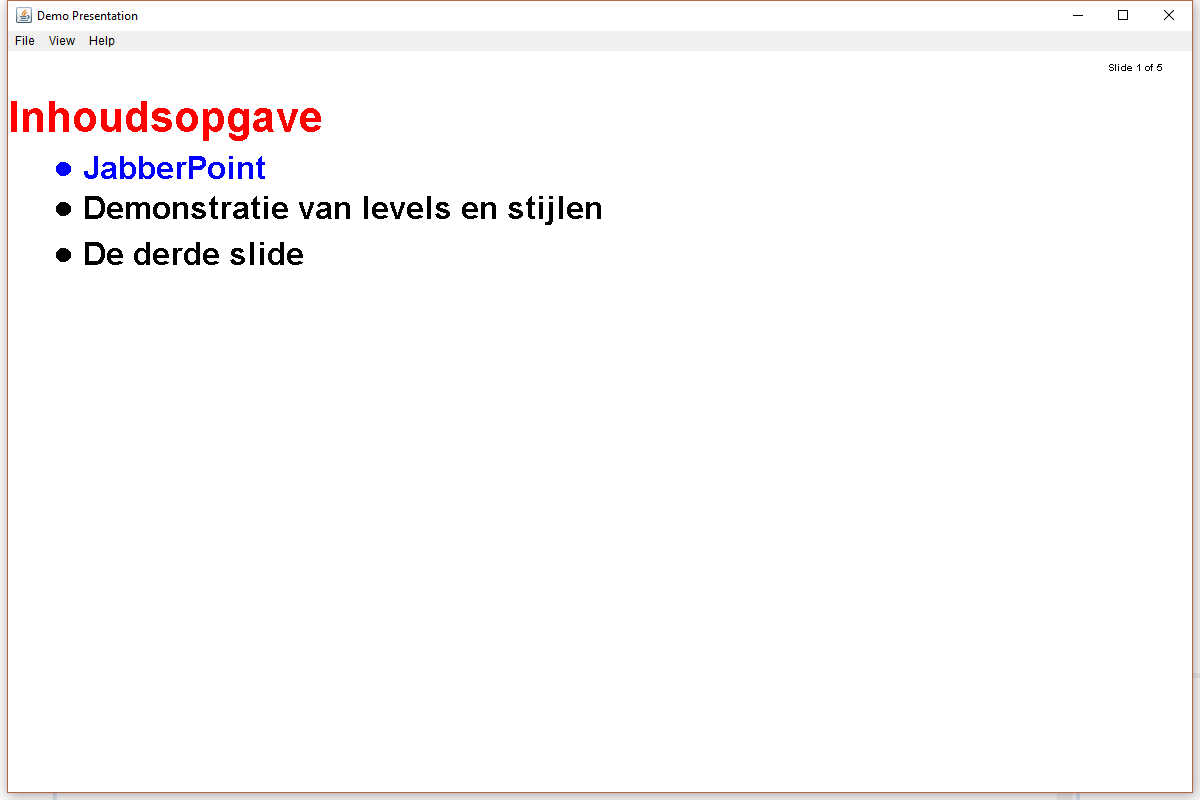
\includegraphics[width=\textwidth]{Screenshots/master.png}
			\end{figure}

		\subsubsection{Traceerbaarheid van eisen}
			In deze sectie geef ik onderdelen van het ontwerp aan die verantwoordelijk zijn om de eisen (zie sectie~\ref{sec:probleemanalyse}) te realiseren.
			Dit geeft dus de relatie tussen probleemanalyse en ontwerp.

			\begin{itemize}
				\item De \code{Accessor}-klassen zijn verantwoordelijk voor \reqref{toevoegen}.
				\item De \code{TableOfContentsSlide} klasse is verantwoordelijk voor \reqref{tonen}, \reqref{samenvoegen},
					\reqref{updaten}, \reqref{titel}, \reqref{volgnummers}, \reqref{aanduiding} en \reqref{stijl}.
				\item De \code{Slide} klasse is verantwoordelijk voor \reqref{onderwerpen}.
			\end{itemize}

	\subsection{View}\label{sec:view}
		Het \code{jabberPoint.view} package bevat alle nodige code voor de gebruikersinterface.
		Het klassendiagram van de view wordt in figuur~\ref{diagram:view} getoond.

		\diagram{view}{
			Klassendiagram voor de view-klassen.
			Factories zijn weggelaten.
			Referenties naar controller en model zijn beperkt gehouden voor de duidelijkheid.
		}

		Het element dat het volledige scherm opbouwt is de \code{JabberpointFrame}.
		Deze klasse bevat de twee controllers (zie sectie~\ref{sec:controller}) en de \code{PresentationView}.

		\code{PresentationView} krijgt de presentatie als referentie en is verantwoordelijk om de juiste slide te tonen.
		Om te weten wanneer een nieuwe slide moet worden getoond maak ik gebruik van het \textit{observable-patroon} (zie sectie~\ref{sec:utils}).
		Op het moment dat de \code{update} methode wordt aangeroepen, wordt een nieuwe \code{SlideView} gemaakt via de bijbehorende factory.

		De \code{SlideView} klasse is verantwoordelijk om de slide te tekenen en maakt gebruikt van \code{SlideItemView} instanties.
		Deze kunnen of een \code{BitmapItemView} of een \code{TextItemView} zijn, maar de keuze voor de juiste view gebeurt in de factory (zie sectie~\ref{sec:view-factories})

		Aanvullende documentatie over de klassen en hun verantwoordelijkheden zijn beschikbaar in de Javadoc bij de code (zie sectie~\ref{sec:source}).

		\subsubsection{Factories}\label{sec:view-factories}
			Alle klassen mogen alleen door factories worden gemaakt.
			De factories geven alle nodige dependencies mee op het moment dat de klasse gemaakt wordt (\textit{dependency injection} patroon).
			De view factories worden gegroepeerd in het package \code{jabberPoint.view.factories}.
			Een klassendiagram van dit package wordt in figuur~\ref{diagram:view-factories} getoond.

			De \code{PresentationViewFactory} is verantwoordelijk om \code{JabberPointFrame} te maken met de juiste \code{PresentationView}.
			\code{SlideViewFactory} maakt de implementaties van \code{Slide}.
			\code{SlideItemViewFactory} maakt de implementaties van \code{SlideItemView}.
			Ten slotte maakt \code{StyleFactory} de juiste \code{Style} afhankelijk van de slide en slide-item.

			\diagram{view-factories}{
				Klassendiagram voor de view-factories.\label{diagram:view-factories}
				Details zijn weggelaten voor de duide\-lijk\-heid.
			}

	\subsection{Controller}\label{sec:controller}
		Het \code{jabberPoint.controller} package bevat alle nodige code voor het veranderen van de model via de gebruikersinterface.
		Het klassendiagram wordt in figuur~\ref{diagram:controller} getoond.

		\begin{figure}[!htb]
		 \caption{
			Klassendiagram voor de controller-klassen.\label{diagram:controller}
			Factories zijn weggelaten.
			Referenties naar view en model zijn beperkt gehouden voor de duidelijkheid.
		 }
		 \makebox[\textwidth][c]{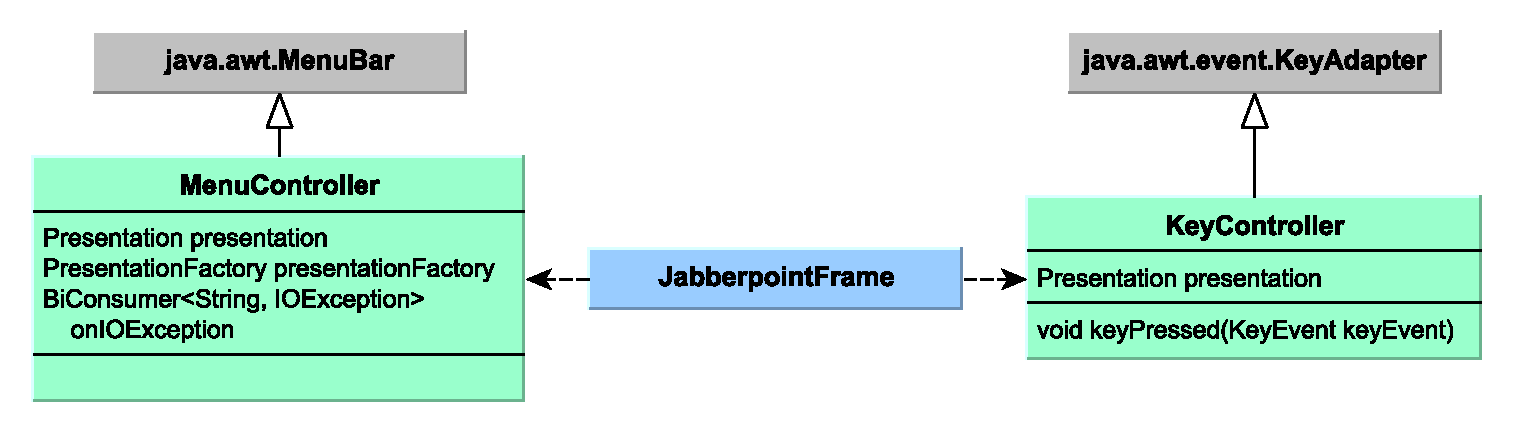
\includegraphics[width=1.3\textwidth]{Diagrams/controller.pdf}}%
		\end{figure}

		Jabberpoint kent twee manieren om de presentatie te navigeren: via het menu of via het toetsenbord.
		Daarom hebben we ook twee controllers: \code{Menu}\-\code{Controller} en \code{KeyController}.
		Beide krijgen een presentatie in de constructors zodat de controllers commando's kunnen doorgeven.
		\code{MenuController} krijgt bovendien een instance van \code{PresentationFactory} omdat deze presentaties moet kunnen openen.
		Hierin kunnen fouten optreden, en \code{MenuController} is niet zelf verantwoordelijk om een foutmelding te tonen.
		Deze worden getoond door de view via de \textit{callback}-functie \code{BiConsumer onIOException}.

		Aanvullende documentatie over de klassen en hun verantwoordelijkheden zijn beschikbaar in de Javadoc bij de code (zie sectie~\ref{sec:source}).

		\subsubsection{Factories}\label{sec:controller-factories}
			Alle klassen mogen alleen door factories worden gemaakt.
			De factories geven alle nodige dependencies mee op het moment dat de klasse gemaakt wordt (\textit{dependency injection} patroon).
			De controller factories worden gegroepeerd in het package \code{jabberPoint.controller.factories}.
			Een klassendiagram van dit package wordt in figuur~\ref{diagram:controller-factories} getoond.

			\diagram[0.8]{controller-factories}{
				Klassendiagram voor de controller-factories.\label{diagram:controller-factories}
				Details zijn weggelaten voor de duide\-lijk\-heid.
			}

	\section{Utils}\label{sec:utils}
		De klassen het \code{utils}-package zijn in een apart package geplaatst omdat ze niet specifiek voor Jabberpoint zijn.
		Het gaat namelijk om de implementatie van het \textit{Observable-patroon}.
		De Java-klassen hiervoor hebben geen typing, waardoor casts nodig zijn.
		Door de toepassing van generics kan dit verbeterd worden.
		
		Het patroon is geïmplementeerd door middel van twee interfaces en één abstracte klasse:
		\begin{itemize}
			\item \code{Observer<ObservedType>} is de interface voor klassen die andere klassen kunnen observeren.
				Deze interface bevat de method \code{update} om updates te krijgen.
			\item \code{Observable<ObservedType>} is de interface voor klassen die geobserveerd kunnen worden.
				Deze interface bevat de methoden \code{addObserver} en \code{notify}\-\code{Observers}.
			\item \code{BaseObservable<ObservedType>} is een abstracte implementatie van \code{Ob}\-\code{servable}.
				Deze implementatie zorgt voor een standaard implementatie van de vereiste methoden.
		\end{itemize}

		Op deze manier kan de presentatie \code{Observable<Slide>} implementeren door \code{BaseObservable<Slide>} uit te breiden.
		View-\textit{observers} implementeren \code{Obser}\-\code{ver<Slide>} om te weten als een nieuwe slide moet worden getoond.
		Het package wordt afgebeeld in het model-diagram (figuur~\ref{diagram:model}, pagina~\pageref{diagram:model}).

\section{Keuzen}\label{sec:keuzen}
    In deze sectie gaan we een aantal vragen door die zijn opgeroepen tijdens het analyseproces.
   
    \question{Welke klasse is verantwoordelijk voor onderwerpen?}
		De inhoudsopgave moet toegang krijgen tot een lijst van onderwerpen in de presentatie.
		In het ontwerp krijgt \code{TableOfContentsSlide} een referentie naar de presentatie en is zelf verantwoordelijk om deze te lezen.
		En alternatief hierop is om de presentatie verantwoordelijk te houden voor de onderwerpen in de slides.
		\code{TableOfContentsSlide} zou dan een dan een onderwerpen-lijst ontvangen.

		De voordelen van deze alternatief zijn:
		\begin{itemize}
			\item De inhoudsopgave hoeft niets te weten van de presentaties.
			\item De presentatie is verantwoordelijk om zijn eigen slides te lezen.
			\item De circulaire referentie wordt opgeheven.
			\item De lijst van onderwerpen kan tussen de verschillende inhoudsopgaven worden gedeeld.
		\end{itemize}

		De nadelen zijn:
		\begin{itemize}
			\item Er komt meer logica in de presentatie die alleen nodig is voor de in\-houds\-op\-gave.
			\item De inhoudsopgaven moeten nog steeds alle items doorlopen om te bepalen welk onderwerp het volgende is.
			\item De methoden die nodig zijn om de slides te lezen bestaan al in de presentatie.
			\item Het is conceptueel correct om een circulaire referentie te hebben, immers een inhoudsopgave moet een overzicht van de presentatie laten zien.
			\item De presentatie klasse wordt nog complexer.
		\end{itemize}

		De keuze om de lijst van onderwerpen in de inhoudsopgave te implementeren geeft dus een betere inkapseling.

    \question{Moet een inhoudsopgave een andere stijl krijgen?}
		De standaard stijl van de slides is niet optimaal voor een inhoudsopgave, alhoewel \reqref{stijl} expliciet aangeeft dat stijlen vrij te bepalen zijn.
		Het is met deze stijl echter niet helemaal duidelijk dat het om een lijst van onderwerpen gaat.
		Door een icoontje toe te voegen aan elke item en steeds dezelfde indentatie te gebruiken, wordt het duidelijker.
		Daarom heb ik aparte stijlen geïmplementeerd via de \code{StyleFactory}.
		Een screenshot van de inhoudsopgave met deze stijl wordt in figuur~\ref{fig:master} getoond (pagina~\pageref{fig:master}).

    \question{Moet de versiegeschiedenis in de bestanden zijn?}
		In de initiële versie van Jabberpoint stond bovenaan in elk bestand een geschiedenis van de versies.
		Met een moderne ontwikkelmethode verandert de code heel snel, de lijst wordt heel lang en niet altijd up-to-date gehouden.
		Bovendien gebruiken we nu een tool die specifiek gemaakt is om code-geschiedenis bij de houden, namelijk Git.
		Daarom heb ik besloten om deze versiegeschiedenis te verwijderen van alle files en deze alleen in Git te houden.

		De auteur-melding is wel gehouden omdat deze kort is en niet zo vaak verandert.
		Git zou dit prima kunnen bijhouden, echter is de historie kwijt toen ik de code importeerde in een nieuwe repository.
		Het is dan netjes om de oorspronkelijke auteurs te benoemen.

    \question{Moet de code worden voorzien van Javadoc?}
		Om software echt onderhoudbaar te maken is het ontwikkelen met ontwerp-patronen niet voldoende.
		Ik ben namelijk van mening dat de documentatie bij de code van essentieel belang is.
		Daarnaast is het schrijven van de bedoeling van een stukje code een belangrijk hulpmiddel om de codekwaliteit te evalueren.
		Daarom heb ik de hele applicatie voorzien van Javadoc op het niveau van klassen en methoden (inclusief parameters).
		De meeste attributen zijn overigens ook gedocumenteerd.

	\question{Is het updaten van Java verstandig?}
		De Jabberpoint applicatie maakte gebruik van Java 1.6.
		Tijdens de refactoring heb ik besloten om de Java-versie te updaten naar 1.8.
		Met deze versie van Java is het gebruik van lambda-functies mogelijk.
		Daardoor was het mogelijk om de controllers veel eenvoudiger te maken.

	\question{Moet lezen en schrijven in een apart package komen?}
		Tijdens het splitsen van Jabberpoint in MVC-packages rees de vraag: waar horen de I/O klassen bij?
		In beschrijvingen van MVC wordt de model vaak beschreven als ``\textit{business logic-related data}''.
		Daarom vind ik dat de \code{Reader} en \code{Writer} klassen in ook in dit package horen, zeker gezien hoe eenvoudig de applicatie is.

		Er zijn nog twee opties mogelijk die ik net zo passend vind:
		\begin{itemize}
			\item Een apart package onder JabberPoint, bijvoorbeeld \code{jabberPoint.io};
			\item Een sub-package van model, bijvoorbeeld \code{jabberPoint.model.io}.
		\end{itemize}

	\question{Moeten overal interfaces worden gedefinieerd?}\label{q:interfaces}
		Een aantal concrete klassen in het ontwerp worden gebruikt door veel andere klassen.
		Bijvoorbeeld de \code{Presentation} klasse heeft veel referenties.
		Voor alle concrete klassen zouden we een interface kunnen definiëren met één implementatie.
		Als resultaat zouden de concrete klassen alleen in de factories voorkomen.

		Echter heb ik ervoor gekozen om geen interfaces te definiëren.
		Het is namelijk simpel in Java om een klasse naar een interface te converteren.
		Elke klasse kan altijd een interface worden zonder de gebruikers van de klasse te veranderen.
		Zo houden we het ontwerp kort en bondig zonder verlies van flexibiliteit.

	\question{Waarom aparte view-klassen voor slide items?}
		In het ontwerp zien we dat de \code{SlideView} werkt met de abstracte \code{Slide} klasse.
		Daarom is geen \code{ContentSlideView} of \code{TableOfContentsSlideView} nodig.
		De slides moeten namelijk op dezelfde manier worden getoond, alleen de inhoud is anders.

		Echter voor de slide-items was een dergelijke constructie niet mogelijk.
		Er is dus een interface \code{SlideItemView} met implementaties \code{TextItemView} en \code{Bitmap}\-\code{ItemView}.
		De slide-items zijn zodanig anders van elkaar dat het niet mogelijk is om op een generieke manier te tekenen.

	\question{Waarom geen abstracte factory?}
		In het cursus-tekstboek worden allerlei soorten factories besproken.
		``Factory'' wordt echter niet benoemdt in de lisjt met patronen (zie chapter 20, bijvoorbeeld page 348).
		De meeste factories in het ontwerp passen daarom niet in de genoemde factory patronen.

		Natuurlijk hebben de factories \textit{factory methods}.
		\code{Presentation} is als \textit{singleton} geïmplementeerd, maar dit wordt geabstraheerd door de factory.
		\code{Style} instanties worden ook één keer gemaakt, maar in verschillende versies: dit lijkt op \textit{object pool}, echter ook dit wordt geabstraheerd.
		Ik vind namelijk belangrijk dat de rest van het systeem niet hoeft te weten hoe de instanties gemanaged moeten worden.

		Een andere optie zou zijn om factories abstract te maken of een interface te definiëren zodat er meerdere varianten van gemaakt kunnen worden.
		Hier geldt echter hetzelfde argument als in sectie~\ref{q:interfaces}: het zou ingewikkelder worden dan noodzakelijk.

		In het geval van \code{StyleFactory} is er wel wat te zeggen voor twee implementaties: één voor inhoud-slides en één voor inhoudsopgave-slides.
		Maar dan moet ergens de beslissing worden genomen over welke factory gebruikt wordt.
		Hiervoor zie ik de volgende opties:
		\begin{itemize}
			\item Een interface voor \code{StyleFactory} en een klasse om de factories te maken (feitelijk een \code{StyleFactoryFactory}).
				Er bestaan dan 4 klassen/interfaces in plaats van één.
			\item De gebruiker van de klasse kiest welke factory gebruikt wordt.
				De \code{Style}\-\code{Factory} is dan niet meer verantwoordelijk voor deze beslissing.
			\item Een abstracte \code{StyleFactory} kent de verschillende implementaties en kan de juiste kiezen (bijvoorbeeld in een static methode).
				Hierdoor ontstaat een circulaire referentie.
		\end{itemize}
		Deze klasse is nog redelijk simpel is en biedt voldoende flexibiliteit.
		Daarom heb ik gekozen voor de oplossing getoond in figuur~\ref{diagram:view} (pagina \pageref{diagram:view}).

	\question{Is het gebruik van constanten een goed idee?}
		Het \code{jabberPoint.view.factories} package bevat de klasse \code{Constants}.
		Hierin bevinden zich de standaard breedte en hoogte van het scherm.
		Deze klasse is gemaakt om code-duplicatie te voorkomen tussen de view-klassen.
		De constante-waarden zijn opgenomen als \code{public final static int} attributen en worden dus niet opgehaald via een methode.

		Een alternatieve optie zou zijn om de constanten \textit{singleton} te maken en de attributen via methoden beschikbaar te maken.
		Zo zouden in de toekomst verschillende implementaties kunnen worden gemaakt.
		Echter worden deze constanten alleen als \textit{preferred} waarden opgenomen in de views.
		De views schalen vervolgens naar de grootte van het venster.
		Het is dan ook niet realistisch te verwachten dat deze verschillende versies moeten krijgen.
		Bovendien worden deze waarden alleen in de factories gebruikt (zie figuur~\ref{diagram:view-factories} op pagina \pageref{diagram:view-factories}).

\section{Sourcecode}\label{sec:source}
	In deze sectie geef ik links naar de verschillende resultaten van de opdracht.
	Alle links betreffen zowel Jabberpoint als dit rapport.
	De broncode is vanzelfsprekend in combinatie met het ontwerp-documentatie in dit document.
	\begin{itemize}
		\item Jabberpoint code:
			\repolink{tree/master/Jabberpoint}\\
			De werking ervan wordt uitgelegd in sectie~\ref{sec:ontwerp}.
		\item \LaTeX ~code:
			\repo{tree/master/Report}{github.com/DanielSchiavini/design-patterns-assignment\-/tree\-/master\-/Report}
		\item CI-configuratie:
			\repolink{blob/master/.travis.yml}
		\item Diagrammen:
			\repo{tree/master/Report/Diagrams}{github.com/DanielSchiavini/design-patterns-assignment\-/tree\-/master\-/Report\-/Diagrams}
		\item Aanpassingen op Jabberpoint:
			\repolink{compare/v0.0.1...master}.
		\item Refactoring:
			\repo{compare/v1.0.0...v2.0.0}{github.com/DanielSchiavini/design-patterns-assignment\-/com\-pare\-/v1.0.0...v2.0.0}
		\item Gegenereerde bestanden:
			\repolink{tree/gh-pages}
		\item Laatste build-rapport van TravisCI:
			\cilink{}
		\item Rapporten van TravisCI:
			\cilink{builds}
	\end{itemize}

\end{document}
